%%%%%%%%%%%%%%%%%%%%%%%%%%%%%%%%%%%%%%%%%%%%%%%%%%%%%%%%%%%%%%%%%%%%%
%%                                                                 %%
%% Please do not use \input{...} to include other tex files.       %%
%% Submit your LaTeX manuscript as one .tex document.              %%
%%                                                                 %%
%% All additional figures and files should be attached             %%
%% separately and not embedded in the \TeX\ document itself.       %%
%%                                                                 %%
%%%%%%%%%%%%%%%%%%%%%%%%%%%%%%%%%%%%%%%%%%%%%%%%%%%%%%%%%%%%%%%%%%%%%

\documentclass[pdflatex,mathphys]{jnl}% Math and Physical Sciences Reference Style

\usepackage{caption}
\usepackage{graphicx}
\usepackage{subcaption}
\captionsetup{justification=justified, font=small}
\usepackage{verbatim}

\usepackage[]{multibib}
\newcites{Meth}{Methods References}

\usepackage{paralist}
\usepackage{lineno}
%\linenumbers

\usepackage{siunitx}
\usepackage{booktabs}
\usepackage{xcolor}

\raggedbottom

\jyear{2026}%

\begin{document}

\title[IMPG]{Implicit pangenome graphs}

\author*[1,2]{\fnm{Andrea} \sur{Guarracino}}\email{aguarracino@tgen.org}
\author[3]{\fnm{Bryce} \sur{Kille}}
\author[]{\fnm{...}}
\author*[1]{\fnm{Erik} \sur{Garrison}}\email{egarris5@uthsc.edu}

\affil[1]{Department of Genetics, Genomics and Informatics, University of Tennessee Health Science Center, Memphis, TN 38163, USA}
\affil[2]{Bioinnovation and Genome Sciences, The Translational Genomics Research Institute (TGen), Phoenix, AZ 85004, USA}
\affil[3]{Illumina Inc., San Diego, CA 92122, USA}

%%==================================%%
%% sample for unstructured abstract %%
%%==================================%%

\abstract{
Querying genomic relationships across hundreds of genomes currently requires either constructing computationally expensive graph structures or using projection tools limited to pairwise mappings between individual genomes. Here we introduce implicit pangenome graphs, a framework that treats pairwise alignments as a queryable pangenome representation, making population-scale analysis accessible on commodity hardware without upfront graph construction.
}

\keywords{pangenomes, pangenome graphs, genome alignment, transitive queries, coordinate projection, population genomics}

\maketitle

%%==================================%%
%%          MAIN TEXT               %%
%%  No section headings allowed     %%
%%==================================%%

Whole-genome alignments are a foundational data layer for pangenomics \cite{computational2018, Eizenga2020b, Paten2017}, yet current workflows treat them as intermediates consumed during graph construction \cite{Garrison2024, Hickey2023}. We propose that the alignment collection itself---together with the transitive relationships it encodes---constitutes a directly queryable pangenome representation. Operating in this alignment space, we can project coordinates transitively across genomes, partition the pangenome along alignment connectivity, and materialize explicit graphs only when needed for specific regions of interest. As high-quality assemblies are now routinely produced for hundreds to thousands of individuals \cite{Liao2023, Wang2022}, this alignment-first approach avoids the substantial computation required for monolithic graph construction at population scale.

Pairwise alignments inherently define a variation graph: positions matched transitively across alignments correspond to shared nodes in a graph that losslessly encodes both the sequences and their relationships \cite{garrison2023seqwish}. The pangenome graph is thus implied by the alignments, even when it is never constructed. Graph construction methods---seqwish \cite{garrison2023seqwish}, Cactus \cite{Paten2011cactus}, TBA/MULTIZ \cite{Blanchette2004}---exploit this property to build pangenome graphs and multiple alignments, but require materializing the complete structure before any region can be examined. Coordinate projection tools such as liftOver \cite{Kuhn2013ucsc} and paftools \cite{Li2018minimap2} operate at query time but map positions between only two genomes; halLiftover \cite{Hickey2013hal} achieves multi-hop projection but requires a pre-computed hierarchical alignment. No existing tool exploits this transitive structure at query time directly from pairwise alignments, without first constructing a graph or hierarchical alignment.

IMPG (Implicit Pangenome Graph) operates directly on pairwise alignments as implicit graph structures (Figure~\ref{fig:concept}A), providing three core capabilities: (a) transitive coordinate projection across all genomes in a pangenome, (b) alignment-based partitioning for distributed graph construction, and (c) on-demand graph materialization for regions of interest. Rather than materializing the full implicit graph, IMPG indexes alignment files using cache-oblivious interval trees \cite{dcjones2020} and traverses them at query time to discover both direct and transitive relationships. Given coordinates on any genome, IMPG projects them onto all other genomes, functioning as a pangenome-wide coordinate liftover. IMPG supports alignments as PAF files (uncompressed and BGZF-compressed), .1aln \cite{myers2025fastga}, and TPA \cite{tpa}---the latter two based on compact tracepoint representations of the alignments---and sequences as FASTA (uncompressed and BGZF-compressed) or AGC archives \cite{deorowicz2023agc}. This flexibility allows integration into existing workflows; supporting tracepoint-based formats and compressed genome archives enables population-scale queries on a single workstation. \textcolor{red}{On the HPRCv2 pangenome (466 haplotypes, 389\,M pairwise alignments in 466 per-file TPA files), IMPG indexes all alignments in X\,minutes and queries a 6\,Mbp region in under 2 seconds, with peak memory of X\,MiB (Supplementary Table~1). Transitive queries from a non-reference haplotype reach all 466 assemblies through multi-hop traversal---from X haplotypes (direct) to 466 (transitive)---demonstrating that the implicit index captures pangenome-wide connectivity (Extended Data Figure~\ref{fig:transitive_reach}). The complete ready-to-query representation of 466 haplotypes---per-file TPA alignments (23.3\,GiB), bidirectional indexes (14.7\,GiB), and AGC archive (3.1\,GiB)---totals 42.5\,GiB (Supplementary Table~1).} The entire human pangenome fits on a laptop disk and can be queried in seconds with minimal memory; no decompression or graph loading step is required.

As pangenome datasets grow to hundreds or thousands of haplotypes, monolithic graph construction becomes intractable: memory, computation, and time scale super-linearly with the number of sequences. Partitioning is essential, but existing approaches operate at whole-sequence granularity. Chromosome-based partitioning assigns entire contigs by chromosome identity; community-based approaches such as PGGB's Leiden clustering \cite{Garrison2024} assign entire contigs to communities based on sequence-similarity networks. Neither can split a contig: if one region of a contig is homologous to chromosome 1 and another to chromosome 5, the entire contig is forced into one partition.

IMPG introduces alignment-based partitioning, which operates at aligned-interval granularity (Figure~\ref{fig:concept}B). The \texttt{partition} command uses sliding windows of transitive queries to divide the pangenome into segments sharing alignment connectivity, and critically, it can split a single contig across multiple partitions at alignment boundaries. This naturally handles cases where different regions of a contig belong to different genomic contexts---including translocations, inter-chromosomal rearrangements, and fragmented assemblies---without requiring special-casing or forcing the entire contig into one partition.

This partitioning splits the pangenome into manageable chunks for any downstream analysis---similarity computation, sequence extraction, genotyping, or graph construction. For graph construction, each partition is processed independently by any tool---PGGB, vg \cite{Garrison2018}, or custom pipelines---distributing computation and memory across nodes; the \texttt{lace} command then merges the resulting subgraphs into a unified GFA or VCF. When a researcher needs to study region-specific variation---visualizing a complex structural variant, inspecting bubble structures, or calling variants against local topology---IMPG can materialize graphs on demand via three built-in engines: seqwish-based graph induction \cite{sweepga, garrison2023seqwish}, POA via SPOA \cite{Vaser2017}, and a recursive divide-and-conquer engine that chunks homologous sequences, builds POA sub-graphs in parallel, and laces them into a single variation graph. The \texttt{align} command supports this by generating sparsified alignment sets guided by Erd\H{o}s--R\'enyi connectivity thresholds \cite{erdos1959random}.

IMPG is already production infrastructure for structural genotyping. The COSIGT pipeline \cite{bolognini2026cosigt} uses \texttt{impg query} to project locus coordinates onto all haplotypes and \texttt{impg refine} to optimize locus boundaries, then constructs local pangenome graphs for genotyping, demonstrating that alignment-space operations can underpin population-scale genotyping of complex variation.

To illustrate IMPG's capacity for rapid population-scale exploration, we investigated a tandem repeat cluster at chromosome 11q23 that Li et al.\ \cite{Li2023} identified as bound by the Epstein--Barr virus EBNA1 protein, inducing chromosomal fragile site breakage. The original study examined four long-read genomes---two Ashkenazi and two Chinese---and reported a $\sim$2.6-fold difference in repeat copy number between the two groups. Using IMPG, we queried this $\sim$21\,kb locus across all 466 HPRCv2 haplotypes in seconds (Figure~\ref{fig:ebv}). Across five superpopulations, repeat region lengths range from 19,941 to 24,468\,bp (1.2-fold) and EBNA1-like motif counts from 446 to 551 per haplotype (1.2-fold), with identical median values across all superpopulations. The apparent $\sim$2.6-fold population difference reported from four genomes is not supported at population scale: variation at this locus is continuous across ancestries, not a discrete two-group difference, illustrating how small sample sizes can mischaracterize structural variation at clinically relevant loci.

More broadly, implicit pangenome graphs introduce a new layer in the pangenome analysis stack. Rather than requiring a single monolithic construction step, the alignment-space framework lets users query, partition, and extract regions on demand, then selectively invoke graph construction only where explicit topology is needed---for bubble enumeration, snarl decomposition, or graph-aware variant calling via tools like Minigraph-Cactus \cite{Hickey2023} or personalized pangenome references \cite{Siren2024}. IMPG can supply these builders with partitioned input through its partition-lace pipeline, or materialize graphs on demand for specific loci. The two representations are complementary: alignment space provides the upstream infrastructure for exploration and partitioning, while graph space provides the downstream topology for variant-aware analyses.

IMPG's projection accuracy is determined by the quality of the input alignments: given correct alignments, exact-mode queries---which traverse full CIGAR strings (PAF) or reconstruct them via wavefront alignment from tracepoints (.1aln/.tpa)---produce base-exact coordinates by construction. For tracepoint-based formats, an approximate query mode bypasses CIGAR reconstruction entirely, estimating projected boundaries from tracepoint segment coordinates; this is faster but boundaries may differ from exact projections by up to the tracepoint segment size per hop (e.g., $\leq$100\,bp for fixed-spacing tracepoints; \textcolor{red}{Supplementary Table~X}). Regions absent from input alignments cannot be recovered. The incremental design means each new assembly requires alignment against only a spanning subset of existing haplotypes, not a complete rebuild---enabling continuous growth of the pangenome index. Looking forward, transitive queries yield pairwise similarity across indexed haplotypes, opening the possibility of computing population genetics summary statistics directly from alignment space without decomposing variation into biallelic sites. By operating in alignment space, IMPG makes it possible to study sequence variation across populations at scale without requiring upfront graph construction---bridging the gap between assembly production and population-level genomic analysis.

\subsection*{Acknowledgments}

We thank the Human Pangenome Reference Consortium for making the HPRCv2 assemblies publicly available.

\subsection*{Author Contributions Statement}

A.G. developed the software, performed benchmarking and analysis, created visualizations, and wrote the manuscript. B.K. contributed to software development. E.G. conceived the project, developed the software, acquired funding, and wrote the manuscript.

\subsection*{Competing Interests Statement}

B.K. is an employee of Illumina. Other authors declare no competing interests.

\subsection*{Funding}

A.G. and E.G. are funded by NSF PPoSS Award \#2118709; NIH R01HG013618; NIH U01HG013760; NIH U01DA057530; NIH U41HG010972; and the Tennessee Center for Integrative and Translational Genomics.

\clearpage
\bibliography{bibliography}

\clearpage

%%==================================%%
%%          FIGURES                 %%
%%==================================%%

\subsection*{Figures}

\begin{figure}[H]
    %\includegraphics[width=\linewidth]{fig/MainFigures/Fig1.pdf}
    \caption{
      \textbf{IMPG: implicit pangenome graph concept and distributed construction.}
      \textbf{A.} Conceptual overview: pairwise alignments implicitly define a graph structure through transitive match relationships. IMPG indexes alignments using cache-oblivious interval trees and discovers sequences related through multi-hop alignment chains without materializing the graph.
      \textbf{B.} Partition-lace pipeline for distributed pangenome construction. Unlike chromosome-based or whole-sequence community approaches, alignment-based partitioning operates at interval granularity: individual contigs can be split across partitions at alignment boundaries, correctly handling translocations and rearrangements. Partitions are independently processed through graph construction or variant calling tools, then merged into unified GFA or VCF files.
    }
    \label{fig:concept}
\end{figure}

\begin{figure}[H]
    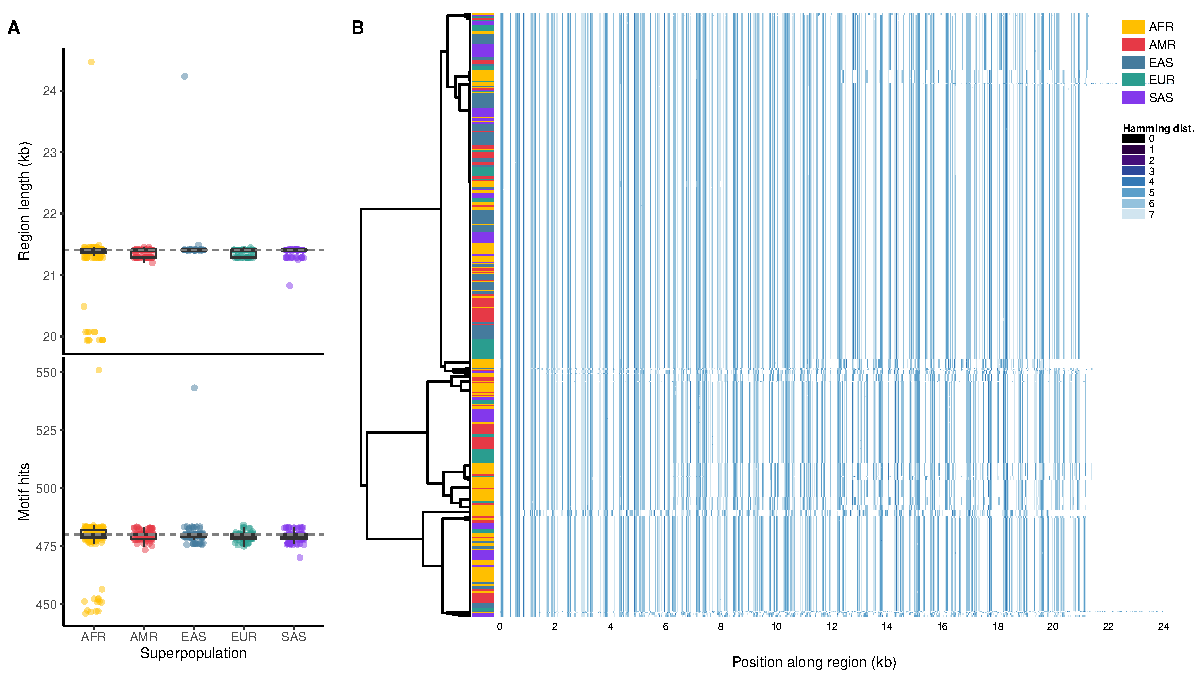
\includegraphics[width=\linewidth]{fig/MainFigures/Fig2.pdf}
    \caption{
      \textbf{EBV-associated tandem repeat polymorphism at 11q23 across 466 human haplotypes.}
      \textbf{A.} Distribution of repeat region lengths (top) and EBNA1-like motif hit counts (bottom) at the chr11q23 tandem repeat cluster across all HPRCv2 haplotypes, colored by superpopulation.
      \textbf{B.} EBNA1-like motif hit positions across all haplotypes, displayed as a binary heatmap (20\,bp bins) with rows ordered by hierarchical clustering (Ward's method on binary distance). Superpopulation annotation is shown as a color bar; the dendrogram reveals structural clusters that do not segregate strictly by ancestry.
    }
    \label{fig:ebv}
\end{figure}

\clearpage

%%==================================%%
%%          METHODS                 %%
%%==================================%%

\section*{Methods}
\label{secMethods}

\setcounter{figure}{0}

Here we provide algorithmic and implementation details not described in the main text.

\subsection*{Overview}

IMPG is implemented in Rust and provides a command-line interface with nine primary operations: \texttt{index} (precompute alignment indices), \texttt{query} (direct and transitive coordinate projection), \texttt{partition} (divide pangenome into non-overlapping segments), \texttt{similarity} (pairwise sequence comparison), \texttt{refine} (optimize locus boundaries), \texttt{align} (generate sparsified alignment pairs), \texttt{graph} (end-to-end graph construction), \texttt{lace} (merge partitioned outputs), and \texttt{stats} (alignment index diagnostics). IMPG is freely available at \url{https://github.com/pangenome/impg} under the MIT license (version 0.4.1 used for all benchmarks).

\subsection*{Core algorithm: implicit pangenome graph}

IMPG exploits a well-established property of pairwise alignments: they inherently define a graph structure through transitive match relationships \cite{Garrison2024, garrison2023seqwish}. This principle underlies multiple alignment methods such as TBA/MULTIZ \cite{Blanchette2004} and T-Coffee \citeMeth{Notredame2000}, which chain pairwise alignments transitively, and explicit graph builders like Cactus \cite{Paten2011cactus}, which compute transitive closure from pairwise alignments. IMPG's contribution is to make this implicit structure efficiently queryable at runtime---discovering sequences connected through intermediate alignments by iteratively following alignment chains---without materializing the graph.

\subsection*{Index structure}

The implementation utilizes cache-oblivious interval trees (coitrees) \cite{dcjones2020} that use a van Emde Boas recursive layout to represent tree structures implicitly using array indices rather than pointers. This layout achieves $O(\log_B n + k/B)$ cache misses for block size $B$, reducing memory overhead while maintaining efficient query performance. Sequence names are mapped to numeric identifiers through a deterministic sorting scheme, ensuring reproducible results. CIGAR strings are packed into compact 32-bit integers, with three most significant bits encoding the operation type and the remaining 29 bits encoding the operation length. Rather than loading all alignment data into memory, IMPG stores byte offsets to CIGAR data in the original files, enabling on-demand retrieval.

The index file structure uses a forest map---a lookup table that maps sequence IDs to their corresponding interval tree locations within the index file. Individual coitrees for each target sequence are stored sequentially, with byte offsets recorded in the forest map at the file's end. This enables lazy loading of specific target trees without parsing the entire index.

By default, each alignment A$\rightarrow$B creates an implicit reverse mapping B$\rightarrow$A, doubling the number of index entries but ensuring every haplotype can serve as a bridge for transitive queries in both directions. Users may opt for unidirectional indexing via \texttt{--unidirectional} for smaller indices at the cost of reduced transitive reach.

\subsection*{Alignment formats}

Beyond PAF (both uncompressed and BGZF-compressed), IMPG supports the .1aln format \cite{myers2025fastga} (ONE alignment format) and TPA (TracePoint Alignment) binary files \cite{tpa}. Tracepoints \cite{tpa} store sparse positional checkpoints that record sequence position deltas at complexity-bounded segment boundaries, achieving substantially more compact storage than text-based PAF. CIGAR strings are reconstructed on demand via wavefront alignment (WFA) \citeMeth{marco2023biwfa} within bounded bandwidth, guaranteeing exact reconstruction when the original sequences are available. For tracepoint-based formats, an approximate query mode bypasses CIGAR reconstruction for fast coordinate-level output, estimating projected boundaries from tracepoint segment coordinates without sequence I/O. Exact-mode queries reconstruct the full CIGAR via WFA \citeMeth{marco2023biwfa} and produce base-exact coordinates. A comparison of interval boundaries between the two modes is provided in Supplementary Table~X.

\subsection*{Multi-file index architecture}

For large distributed datasets, IMPG supports per-file indexing with a unified sequence namespace. Each alignment file has its own .impg index and a serializable cache that stores the unified sequence index together with ID translation tables. Staleness detection based on file size and modification time ensures cache consistency. The indexing mode is selected automatically ($\geq$100 files triggers per-file mode) or controlled via \texttt{--index-mode}. Critically, per-file indexing enables incremental indexing: new files require indexing while existing indices are reused without rebuilding.

\subsection*{Query algorithms}

Basic overlap queries identify all alignments whose target intervals intersect a query range with $O(\log n + k)$ complexity. Query results include projected coordinates computed by traversing CIGAR operations to map target ranges to query coordinates.

Transitive queries iteratively follow alignment chains to discover sequences connected through intermediate alignments. The Erd\H{o}s--R\'enyi random graph model \cite{erdos1959random} provides a heuristic guideline: when pairs are connected with probability $P > (1+\epsilon) \frac{\ln N}{N}$, the resulting random graph is connected with high probability using $O(N \log N)$ rather than $O(N^2)$ edges. Because genomic alignments are not random---they depend on sequence similarity and population structure---this threshold serves as a practical lower bound rather than a formal guarantee. The default traversal depth is two hops (sufficient for reference-bridged datasets) and can be increased via \texttt{--max-depth}. Two traversal strategies are implemented: breadth-first search (BFS) for optimal cache locality and depth-first search (DFS) for fewer overlapping results in dense regions.

\subsection*{Partitioning algorithm}

The \texttt{partition} command iteratively divides the pangenome into non-overlapping partitions using sliding windows of transitive queries, maintaining masked regions (already partitioned) and missing regions (not yet partitioned). Crucially, the algorithm operates at aligned-interval granularity: a single contig can be split across multiple partitions at alignment boundaries, with each interval assigned to the partition containing its homologous context. The sliding window mechanism scans reference coordinates, collecting transitively connected intervals into candidate partitions, and advances past already-partitioned (masked) regions. Four selection strategies control partition characteristics: longest (minimizes partition count), total (greatest unpartitioned content), sample (maximizes sample representation), and haplotype (maximizes haplotype diversity).

\subsection*{Comparison with partitioning approaches}

Three approaches to pangenome partitioning differ in the granularity at which they assign sequences. Chromosome-based partitioning assigns contigs by chromosome identity, assuming synteny; this fails for translocations, inter-chromosomal rearrangements, and fragmented contigs that cannot be cleanly assigned to a single chromosome. Community-based partitioning, as implemented in PGGB's Leiden clustering \cite{Garrison2024}, operates on sequence-similarity networks at whole-sequence granularity: entire contigs are assigned to communities, so a contig with regions homologous to different genomic contexts is forced into one partition. PGGB's documentation notes that translocations may be conflated with syntenic regions under this approach, and sequence similarity serves as a proxy for homology rather than a direct measure. IMPG's alignment-based partitioning operates at the level of aligned intervals: contigs are split at alignment boundaries, and intervals from the same contig are routed to different partitions when they align to different genomic contexts. This handles translocations naturally without special-casing and does not require synteny assumptions or whole-sequence similarity networks. The three approaches reflect different design goals---chromosome-based partitioning prioritizes simplicity, community-based partitioning balances scalability with sequence-level grouping, and alignment-based partitioning maximizes granularity at the cost of requiring indexed pairwise alignments.

\subsection*{Similarity analysis}

The \texttt{similarity} command computes pairwise similarity coefficients between sequences in specified genomic regions. Overlapping sequences are extracted, aligned via POA (SPOA) to produce a multiple sequence alignment, and pairwise similarities computed from column-wise intersection counts. Three metrics are supported: Jaccard ($J = |A \cap B| / |A \cup B|$), Cosine ($\cos = |A \cap B| / \sqrt{|A| \cdot |B|}$), and Dice ($D = 2|A \cap B| / (|A| + |B|)$). The resulting matrices can be processed through integrated PCA or MDS implementations with adaptive polarization for genome-wide consistency.

\subsection*{Locus refinement}

The \texttt{refine} command optimizes genomic loci to maximize the number of entities (sequences, samples, or haplotypes) spanning both boundaries. This is particularly valuable for structural variant analysis where loci should avoid terminating within large insertions or deletions. The algorithm explores asymmetric left and right boundary expansions with configurable extension steps.

\subsection*{Alignment generation}

The \texttt{align} command generates sparsified pairwise alignment sets using connectivity targets derived from the Erd\H{o}s--R\'enyi model. Four strategies are supported: exhaustive ($O(N^2)$), random subsampling, connectivity-probability (default: 0.99), and tree-based sampling combining MinHash nearest-neighbor and stranger-joining pair selection \cite{sweepga}. In joblist mode, the command emits alignment commands for cluster distribution; direct execution via the embedded FastGA aligner is supported for smaller datasets.

\subsection*{Graph building engines}

IMPG provides three graph construction engines, selectable via \texttt{--engine}:

\textbf{Seqwish engine} (default for \texttt{graph}). The \texttt{graph} command provides end-to-end pangenome graph construction from FASTA sequences: FastGA alignment via sweepga \cite{sweepga}, filtering (scaffold chaining, cardinality control, identity and overlap filtering), seqwish-based graph induction \cite{garrison2023seqwish}, and GFA sorting via path-guided stochastic gradient descent.

\textbf{POA engine.} For small regions ($\leq$10\,kbp), SPOA-based \cite{Vaser2017} partial order alignment produces a variation graph in a single pass. This engine applies padded POA (described below) when boundary context is needed.

\textbf{Recursive engine} (default for \texttt{query} and \texttt{partition} GFA output). A divide-and-conquer strategy that constructs variation graphs from sets of homologous sequences through recursive partitioning, parallel POA, and sub-graph lacing. The algorithm proceeds as follows:

\begin{enumerate}
\item \textit{Recursion decision.} If the longest sequence span is at most \texttt{poa\_threshold} (default 1\,kbp) or recursion depth reaches \texttt{max\_depth} (default 10), the base case applies directly. When the number of sequences exceeds \texttt{seqwish\_threshold} (default 500), seqwish is used instead of POA to avoid $O(N \cdot L)$ memory consumption.

\item \textit{Alignment and anchor selection.} An all-vs-all alignment is computed via sweepga with $k$-mer frequency scaled to the sequence count ($N \times 10$, ensuring seeds are retained among $N$ nearly-identical sequences). The longest sequence serves as the anchor.

\item \textit{Chunk partitioning.} The anchor is divided into overlapping windows of \texttt{chunk\_size} (default 5\,kbp) with \texttt{padding} (default 100\,bp) overlap on each side. For each window, alignment records are used to project the anchor's coordinate range onto every other sequence via linear interpolation through alignment blocks, supporting both forward and reverse strand mappings. Sequences lacking alignment to the anchor are included in every chunk as a fallback.

\item \textit{Parallel recursion.} Chunks are processed in parallel via rayon, each recursively invoking the engine.

\item \textit{Sub-graph lacing.} The resulting sub-GFAs are unified into a single graph. Node IDs are translated into a global namespace. Path ranges---encoded in path names as \texttt{name:start-end}---are sorted, deduplicated, and overlap-trimmed at chunk boundaries by walking node sequences to identify the overlap region and splitting or removing nodes accordingly. Contiguous ranges are linked with new edges, and unused nodes are removed.
\end{enumerate}

\noindent\textit{Padded POA.} When the POA base case operates on chunk boundaries, alignment quality can degrade at the edges of subsequences. Padded POA addresses this by extending each sequence by a configurable number of flanking bases on each side before running SPOA. After alignment, an MSA is generated to identify the columns corresponding to padding: for each sequence, the algorithm walks MSA columns consuming non-gap characters until the left-padding count is exhausted, then similarly from the right. The core column range is defined as the intersection across all sequences. A fresh SPOA graph is then built from only the core (non-padding) subsequences, ensuring that boundary artifacts from the padding context do not propagate into the final graph. In the recursive engine, padding is handled at the chunk-partitioning level (overlapping windows) rather than at the POA level, and the lacing step trims the resulting overlaps.

\subsection*{Alignment statistics}

The \texttt{stats} command reports diagnostics on alignment indices: the number and total length of query and target sequences, overlap counts (total, mean, and median per sequence), the five most-connected target sequences, and bridge genome coverage---the fraction of target sequences that also appear as queries, indicating bidirectional index completeness. A warning is emitted when bridge coverage falls below 50\% of targets, suggesting the index may benefit from rebuilding without \texttt{--unidirectional}. The \texttt{--list-sequences} flag prints a tab-separated list of sequence names and lengths.

\subsection*{Output merging}

The \texttt{lace} command combines partition outputs: GFA merging resolves node ID conflicts and maintains path continuity; VCF merging performs coordinate sorting and contig validation. Output compression is supported in gzip, bgzip, and zstd formats.

\subsection*{Input and output formats}

Input formats: FASTA files and AGC archives \cite{deorowicz2023agc} for sequences; PAF (uncompressed/BGZF), .1aln \cite{myers2025fastga}, and TPA \cite{tpa} for alignments. Output formats: BED, BEDPE, PAF (intervals and alignments); GFA via seqwish, POA, or recursive engines; MAF (multiple alignment); FASTA with optional gap characters and alignment information.

\subsection*{Benchmarking}

We benchmarked IMPG on 389,234,668 pairwise alignments in 466 TPA files (one per target haplotype, 23.27\,GiB on disk) from 25,221 random haplotype pairs sampled from the Human Pangenome Reference Consortium Phase~2 pangenome (HPRCv2, 466 haplotypes: 464 HPRC haplotypes plus CHM13 and GRCh38 references). All benchmarks were run on an AMD Ryzen 7 PRO 7840U workstation (16 threads) with 57\,GiB RAM using IMPG v0.4.1.

\textcolor{red}{Index creation across all 466 per-file TPA files completed in X\,minutes using 16 threads, producing bidirectional indexes totaling 14.7\,GiB. Bidirectional indexing produced X\,M entries from 389\,M records (not exactly doubled because self-alignments are not duplicated).}

\textcolor{red}{For querying the 6\,Mbp MHC region (CHM13\#0\#chr6:28000000-34000000): direct queries completed in X\,s (TPA approximate) with X\,MiB peak memory; transitive queries in X\,s (TPA approximate).} The complete ready-to-query representation---per-file TPA alignments (23.3\,GiB), bidirectional indexes (14.7\,GiB), TPA auxiliary indexes (1.4\,GiB), and AGC archive (3.1\,GiB)---totals 42.5\,GiB. This is the full representation of 466 human haplotypes: no decompression, graph construction, or additional preprocessing is required to begin querying. At approximately 93\,MiB per haplotype, the per-haplotype cost suggests that datasets of thousands of haplotypes remain tractable on commodity storage.

\subsection*{EBV repeat locus analysis}

We queried the EBNA1-binding tandem repeat cluster at chromosome 11q23, reported at GRCh38 chr11:114,604,212--114,625,620 by \cite{Li2023}. Since GRCh38 is included among the 466 assemblies in the dataset, we queried directly from GRCh38 coordinates using \texttt{impg query} in transitive mode with approximate coordinate projection, projecting through all available alignment paths (all-vs-GRCh38, all-vs-CHM13, and a random subset of all-vs-all) to reach all haplotypes. Repeat region lengths were computed from the projected intervals as the sum of all interval spans per haplotype. To quantify repeat copy number, we extracted FASTA sequences for all projected intervals using \texttt{impg query} with AGC-backed sequence retrieval and counted occurrences of the 18-bp EBNA1 binding motif (GGGTAGCATATGCTACCC) and its reverse complement within Hamming distance $\leq$\,7 in each haplotype's sequence. Superpopulation assignments for HPRC samples were derived from the HPRC Release~2 sample metadata (\url{https://github.com/human-pangenomics/hprc_intermediate_assembly}) using standard 1000 Genomes population-to-superpopulation mappings. Analysis scripts are available in the repository (\texttt{paper-nmeth/scripts/run\_ebv\_analysis.sh}).

\subsection*{Data Availability}

IMPG is freely available at \url{https://github.com/pangenome/impg} under the MIT license (version 0.4.1 used for all benchmarks). Benchmark scripts are included in the repository. Input assemblies are from the HPRCv2 release (\url{https://humanpangenome.org}); the CHM13v2.0 reference is available from the T2T Consortium (\url{https://github.com/marbl/CHM13}). Pre-computed alignments, TPA files, and IMPG indexes for the HPRCv2 dataset are available at Zenodo (DOI: \url{https://doi.org/10.5281/zenodo.XXXXXXX}).

\subsection*{Code Availability}

All source code is available at \url{https://github.com/pangenome/impg} under the MIT license. Scripts for reproducing all analyses presented in this paper are included in the repository.

\bibliographystyleMeth{mathphys}
\bibliographyMeth{bibliographyMeth}

\clearpage

%%==================================%%
%%       SUPPLEMENTARY ITEMS        %%
%%==================================%%

\begin{description}
    \item[\textbf{A.}] \textbf{Extended Data Figures}
    \item[\textbf{B.}] \textbf{Supplementary Tables}
    \item[\textbf{C.}] \textbf{Supplementary Figures}
\end{description}

\section{Extended Data Figures}

\begin{figure}[H]
    %\includegraphics[width=\linewidth]{fig/ExtendedDataFigures/Extended_Data_Fig1.pdf}
    \caption{
      \textbf{IMPG index architecture.}
      \textbf{A.} Cache-oblivious interval trees index pairwise alignments by target coordinates, enabling efficient queries without explicit graph construction.
      \textbf{B.} Index file structure with forest map for lazy loading of target-specific trees.
    }
    \label{fig:architecture}
\end{figure}

\begin{figure}[H]
    %\includegraphics[width=\linewidth]{fig/ExtendedDataFigures/Extended_Data_Fig2.pdf}
    \caption{
      \textbf{Transitive query reach from a non-reference haplotype.}
      \textcolor{red}{Querying the MHC region from a non-reference haplotype (HG00097\#1) using the per-file TPA dataset (466 files). Direct query recovers X haplotypes (X intervals); transitive query discovers all 466 assemblies (X intervals), demonstrating that the implicit index captures pangenome-wide connectivity.}
    }
    \label{fig:transitive_reach}
\end{figure}


\section{Supplementary Tables}

\begin{table}[H]
\centering
\caption{\textcolor{red}{IMPG performance on HPRCv2 alignments (466 haplotypes: 464 HPRC + CHM13 + GRCh38; 389\,M pairwise alignments in 466 per-file TPA files). Queries target the 6\,Mbp MHC region (CHM13\#0\#chr6:28000000-34000000). All benchmarks on a 16-core AMD Ryzen 7 PRO 7840U workstation with 57\,GiB RAM running IMPG v0.4.1.}}
\label{tab:benchmarks}
\begin{tabular}{@{}lc@{}}
\toprule
\textbf{Metric} & \textbf{TPA (466 per-file)} \\
\midrule
Alignment records & 389\,M \\
Alignment size on disk & 23.3\,GiB \\
Index size (bidirectional)$^{\dagger}$ & 14.7\,GiB \\
\textcolor{red}{Indexed entries (bidirectional)$^{\dagger}$} & \textcolor{red}{X\,M} \\
\textcolor{red}{Index time (16 threads)} & \textcolor{red}{X\,min} \\
\textcolor{red}{Direct query time} & \textcolor{red}{X\,s} \\
\textcolor{red}{Transitive query time} & \textcolor{red}{X\,s} \\
\textcolor{red}{Peak memory (query)} & \textcolor{red}{X\,MiB} \\
\midrule
\multicolumn{2}{@{}l@{}}{\textit{Complete ready-to-query representation}} \\
TPA alignments & 23.3\,GiB \\
Bidirectional indexes & 14.7\,GiB \\
TPA auxiliary indexes & 1.4\,GiB \\
AGC archive & 3.1\,GiB \\
\textbf{Total} & \textbf{42.5\,GiB} \\
\bottomrule
\multicolumn{2}{@{}l@{}}{\footnotesize $^{\dagger}$Sum across 466 independent per-file indexes; each record indexed as both forward and reverse.}
\end{tabular}
\end{table}

\end{document}
